\documentclass[12pt,a4paper]{article}
\usepackage[a4paper,margin=0.8in,footskip=0.25in]{geometry}

\usepackage{graphicx}

\usepackage{mathtools}
\usepackage{physics}

\usepackage{fontspec} % 加這個就可以設定字體
\usepackage{xeCJK} % 讓中英文字體分開設置

\setCJKmainfont{標楷體} % 設定中文的字型,可以直接輸入系統裡有的字型
% \setmainfont{Times New Roman}

\newfontfamily{\Arial}{Arial}
\newfontfamily{\Calibri}{Calibri}
\newfontfamily{\Times}{Times New Roman}

\newCJKfontfamily\Kai{標楷體} % 定義指令\Kai則切換成標楷體
\newCJKfontfamily\Hei{微軟正黑體} % 定義指令\Hei則切換成正黑體
\newCJKfontfamily\NewMing{新細明體} % 定義指令\NewMing則切換成新細明體

\XeTeXlinebreaklocale "zh" % 這二行,中文才能自動換行
\XeTeXlinebreakskip = 0pt plus 1pt

\title{ML Foundation: HW3}
\author{b04902053 鄭淵仁}

\begin{document}
\maketitle
\section{}

TODO: insert screenshot here.

\section{}

First, we prove ${H}^{2} = H$ :
\[
	\begin{aligned}
		{H}^{2} &= {(X {({X}^{T}X)}^{-1} {X}^{T})} ^ {2} \\
				&= (X {({X}^{T}X)}^{-1} {X}^{T}) (X {({X}^{T}X)}^{-1} {X}^{T}) \\
				&= X {({X}^{T}X)}^{-1} [ ({X}^{T} X) {({X}^{T}X)}^{-1} ] {X}^{T} \\
				&= X {({X}^{T}X)}^{-1} {X}^{T} \\
				&= H
	\end{aligned}
\]

Now we can prove that ${(I-H)}^{2} = (I-H)$ :
\[
	\begin{aligned}
		{(I-H)}^{2} &= {I}^{2} - 2IH + {H}^{2} \\
					&= I - 2H + H \\
					&= I - H
	\end{aligned}
\]

\section{}

TODO: 看不懂題目在寫什麼?QQ

\section{}

\[
	\hat{{E}_2}(\Delta u,\Delta v)
		= E(u, v) + \nabla E(u, v) \cdot (\Delta u, \Delta v)
		+ \frac{1}{2} {(\Delta u, \Delta v)}^{T} {\nabla}^{2}E(u, v) (\Delta u, \Delta v)
\]
Let
\[
	\left\{
		\begin{aligned}
			0 = \pdv{\hat{{E}_2}(\Delta u,\Delta v)}{\Delta u}
				&= \pdv{E}{u} + \frac{1}{2}\left( 2 \pdv[2]{E}{u} \Delta u + 2 \pdv{E}{u}{v} \Delta v \right) \\
				&= \pdv{E}{u} + \pdv[2]{E}{u} \Delta u + \pdv{E}{u}{v} \Delta v \\
			0 = \pdv{\hat{{E}_2}(\Delta u,\Delta v)}{\Delta v}
				&= \pdv{E}{v} + \pdv[2]{E}{v} \Delta v + \pdv{E}{v}{u} \Delta u \\
		\end{aligned}
	\right.
\]
\[
	\left\{
		\begin{aligned}
			0 &= \pdv{E}{u} + \pdv[2]{E}{u} \Delta u + \pdv{E}{u}{v} \Delta v \\
			0 &= \pdv{E}{v} + \pdv[2]{E}{v} \Delta v + \pdv{E}{v}{u} \Delta u \\
		\end{aligned}
	\right.
\]
We can combine the two equations to only one equation by one vector.
\[
	\begin{aligned}
		0 &= \nabla E(u, v) + {\nabla}^{2} E(u, v) \cdot (\Delta u, \Delta v) \\
		- {\nabla}^{2} E(u, v) \cdot (\Delta u, \Delta v) &= \nabla E(u, v) \\
		(\Delta u, \Delta v) &= - {\left({\nabla}^{2} E(u, v)\right)}^{-1} \nabla E(u, v)
	\end{aligned}
\]

\section{}

\section{}

\section{}

\begin{figure}[h!]
  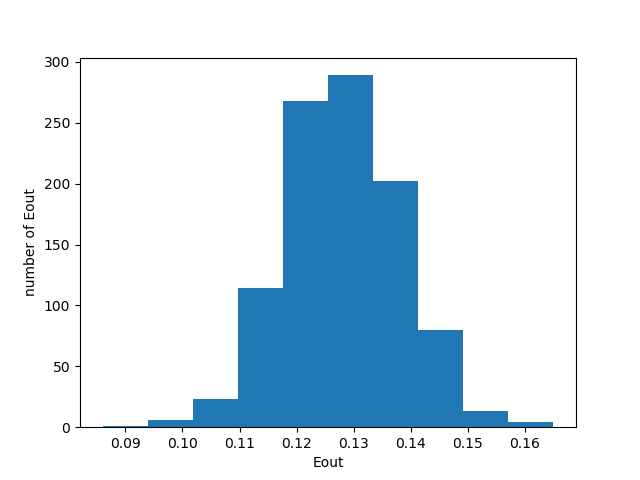
\includegraphics[width=\linewidth]{code/q7.png}
  \caption{Histogram of ${E}_{out}$}
  \label{fig:q7}
\end{figure}

Figure \ref{fig:q7} shows the histogram of ${E}_{out}$.

\end{document}
